\documentclass[12pt]{article}
\usepackage{amsmath, fullpage}
\usepackage{graphicx}
\graphicspath{ {./images/} }

\begin{document}

\title{Causalidad}
\author{Jesus H. Abundis}
%\date{\vspace{-5ex}}
\maketitle
\thispagestyle{empty}

{\large Problemas con retrasos en la red}

\vspace{10pt}
En algunas situaciones, los retrasos de la red puede traer consecuencias no deseadas debido a violaciones del orden.

\begin{figure}[h]
   \centering
   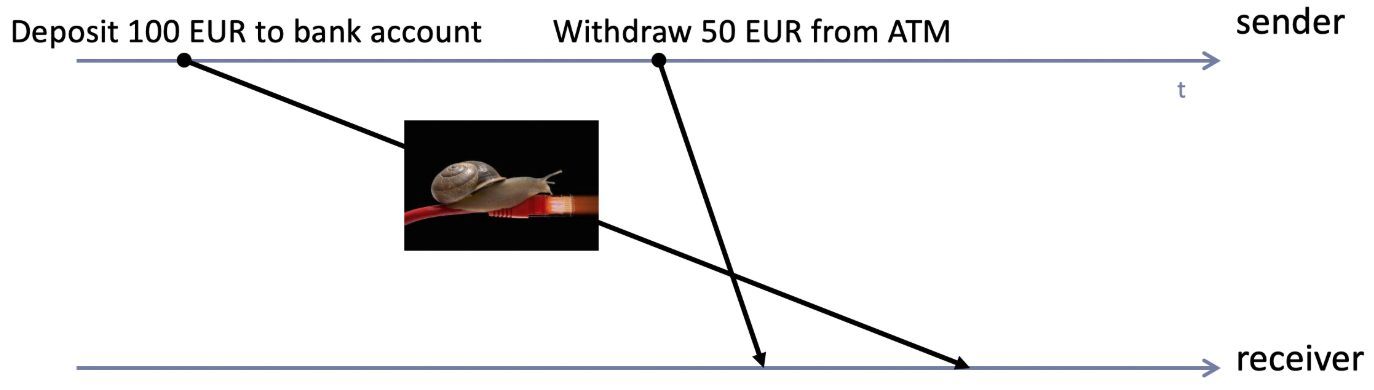
\includegraphics[scale=0.5]{deposito_causalidad.png}
\end{figure}

En el ejemplo superior se envían dos transacciones independientes, 
un depósito de 100 EUR y un retiro de 50 EUR de la misma cuenta bancaria.
Si comenzamos con una cuenta en blanco, 
un retraso significativo del primer mensaje puede ocasionar que la segunda transacción sea cancelada debido a que en este punto el depósito no ha sido procesado.
Esta situación nos señala un problema más profundo.
En muchas aplicaciones, dependemos implícitamente en un principio de orden que un simple canal de comunicación no puede garantizar.


\vspace{15pt}
{\large La búsqueda de la causalidad}

\vspace{10pt}
En en modelo simplificado podríamos asegurarnos que los mensajes se reciben en un orden relativo,
con lo cual nos referimos a que un mensaje enviado primero es también recibido primero por el receptor.
Este modelo se conoce típicamente como First-In-First-Out (FIFO).
Protocolos como el TCP (Transmission Control Protocol) pueden lograr esto dentro de una sola sesión TCP de tal manera que en peor escenario retrasará mensajes fuera de banda y llevará acabo un reordenamiento internamente.

\begin{figure}[h]
   \centering
   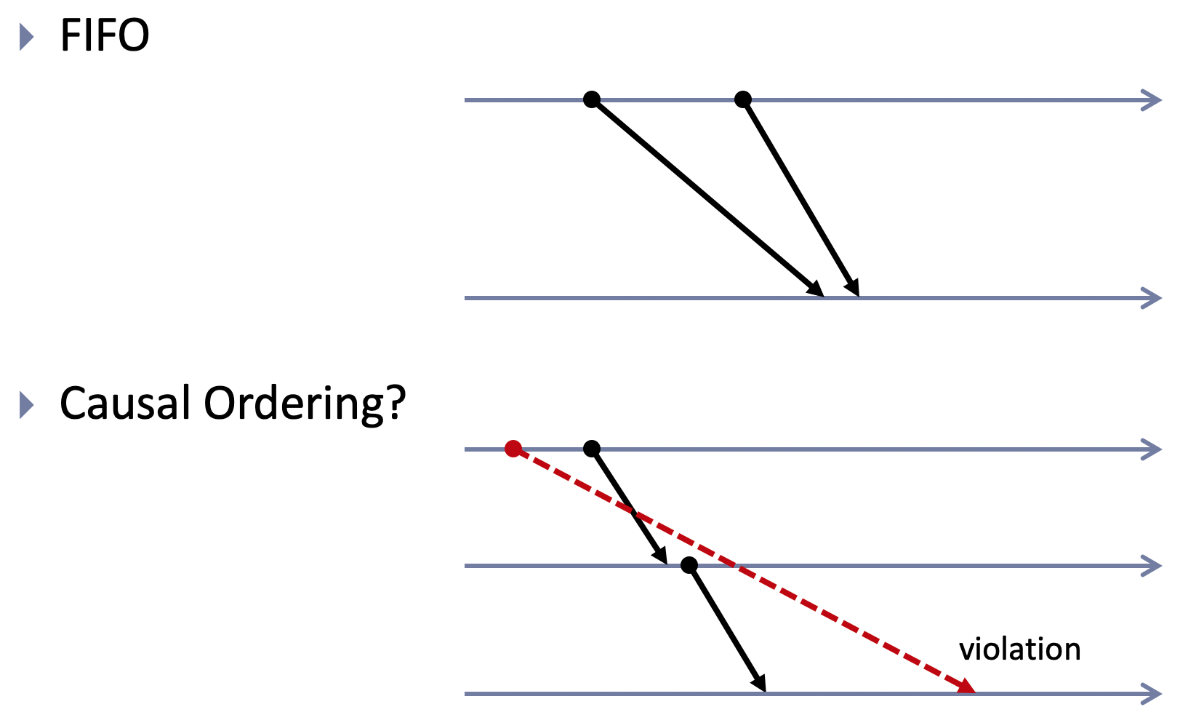
\includegraphics[scale=0.5]{fifo_ordenamiento.png}
\end{figure}
 
Desafortunadamente, el ordenamiento FIFO solo asegura la causalidad entre dos endpoints (puntos finales), 
pero no funciona para más de estos en general.
Como lo muestra la imagen,
todos los mensajes cumplen con el ordenamiento FIFO,
sin embargo,
el mensaje en línea punteada es vencido por la secuencia de mensajes en las líneas continuas.
Desde un punto de vista de punto final a punto final este caso viola el orden causal entre el primer y tercer nodo.

Por causalidad nos referimos a la capacidad de un evento de influenciar a otro, 
lo cuál  en un sistema genérico para el cual desconocemos la semántica de causa y acción, 
debemos asumir que es una propiedad temporal.
Esto significa que, 
si el evento B ocurre después del evento A,
entonces estamos seguros de que este no tuvo un efecto sobre A ya que ocurrio después.
Si B ocurre antes que A,
este pudo tener un efecto sobre A y debemos asumir la causalidad de manera pesimista. 

Sin embargo,
debido a que la red es asíncrona, 
la observación de la llegada de un mensaje da muy poca indicación
sobre cuando fue enviado,
especailmente cuando el mensaje es reenviado a través de uno o más nodos intermedios.
Como hemos visto, puede ser un mensaje retrasado que en realidad ocurrió antes de los mensajes que recibe inicialmente el endpoint.
Como consecuencia,
lograr un orden causal de los mensajes requiere del diseño de protocolos especiales y no puede lograrse mediante canales FIFO que brincan entre nodos. Una solución natural a este problema sería enviar estampas temporales en los mensajes, pero,
como veremos, 
el tiempo es otra instancia de un estado compartido en el cual ya no podemos depender al hacer la transición a un sistema distribuido.


\end{document}
